%\documentclass{jarticle}
%\newcommand{\figref}[1]{\figurename\ref{#1}}
%\newcommand{\tabref}[1]{\tablename\ref{#1}}
%\usepackage[dvipdfmx]{graphicx}
%\begin{document}

%\section{解析}
% この部分にエネルギー解析のみの記載しかしておらず時間解析に関する記述が必要?
\subsection{エネルギー解析}
以上の信号解析で求めらたエネルギー値を元にエネルギースペクトラムを求め,それを元にミッシェルパラメータを求めるための各種解析を行った.まずは各種時間情報を元にスピンの向きに関する考察をし,さらにバックグラウンドの影響を考えてイベントのセレクションを行った.また,エネルギースペクトラムに対するFittingでは検出器内での電磁シャワーによるエネルギー応答を考慮して行列を関数に畳み込んで最小二乗法を適用した.

\subsubsection{スピンの回転に関して}
当初の目標に反して$g$因子測定用に用意した磁場をかけた標的を用いて測定したデータを用いて以下の解析を行った.大きな要因としてはこのデータを元に解析を行っても解析ができることがわかったため,長い時間を測定しイベント量を多く採れたデータを使う方が統計誤差の観点では当然良いため.また,このデータではいろいろな方向のスピン方向の情報を持っているため,$\xi,\delta$といったパラメータの測定も可能であるという事である.以下ではまず時間情報を元にスピン方向のデータが求められる事をみる.時間に関してヒストグラムを出すとg因子の解析で出たような指数関数と三角関数の合わさった形で出てくる.
このままでは例えば$\rho$を求めるためにスピン方向に関して全方向を積分をするために一周期分の時間範囲のデータを取り出しても,指数関数分の減衰があるため,後ろの時間のスピン情報が軽視されるためスピン方向を完全にキャンセルすることができない.これは指数関数の減衰の影響によるものなので,逆にその逆数で重みをつけてやることでその影響をキャンセルできることを確認する.ここではミュオンの崩壊寿命$\tau=2.2\mu s$を既知としてそれぞれのデータに関して$exp(t/\tau)$の重み付けを行った.すると時間情報のヒストグラムは\figref{hatano_fig:oscillation}となった.これは実際の指数関数の影響をキャンセルして,スピンに由来する情報のみを取り出せることを示している.改めて確認するとスピンの向きは三角関数の最大値が$\theta=\pi$,最小値が$\theta=0$に対応する.

\begin{figure}[bht]
  \centering
  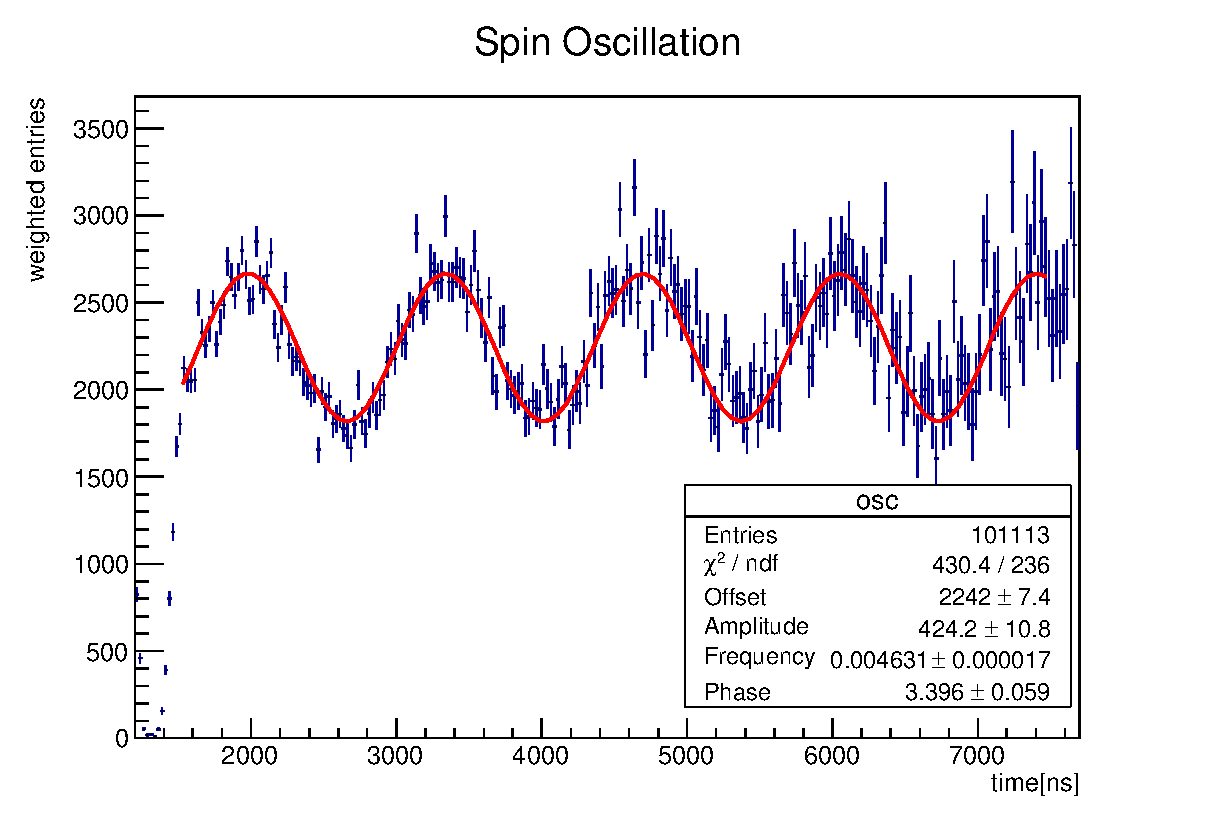
\includegraphics[width=0.8\textwidth]{figure/hatano/oscillation.eps}
  \caption{スピン方向と時間の対応}
  \label{hatano_fig:oscillation}
\end{figure}

以上より,同様の重み付けをした上で適切な時間範囲をとることで任意のスピンに関するエネルギースペクトルを取り出すことができる.

\subsubsection{イベントセレクション}

\subsubsection{検出器の電磁シャワー応答について}
今回の検出器は全吸収型のカロリメータではあるが,検出器内で形成された電磁シャワーで主に$\gamma$線となるものがリークとなるため,必ずしも入射した粒子のエネルギーに対応する形でエネルギーが測定されるわけではなく,低エネルギーの裾をもつ確率分布でエネルギーが与えられる.ただし,この関数形を解析的な形で求めることは難しいので今回はシミュレーション(Geant4)を行って,それらの応答を計算した.結果は\figref{hatano_fig:response}となった.

\begin{figure}[bht]
  \centering
  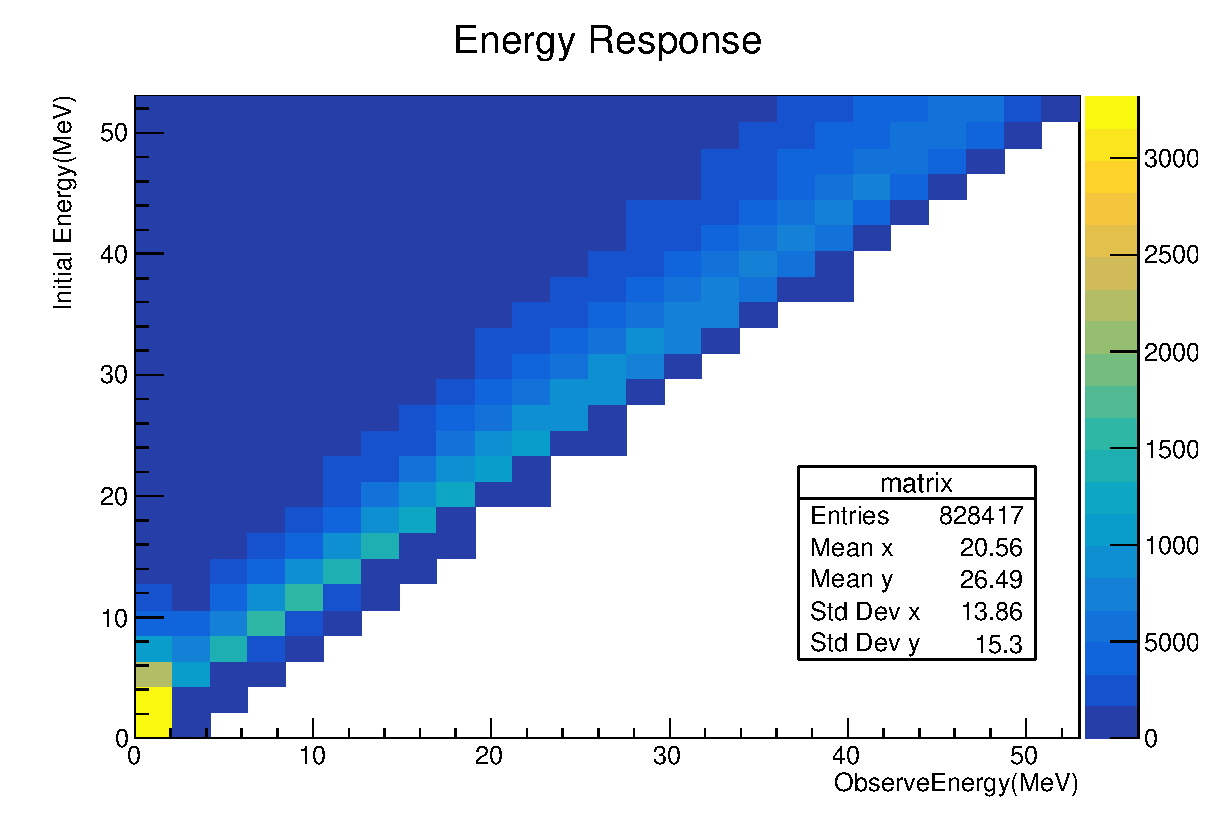
\includegraphics[width=0.8\textwidth]{figure/hatano/response.eps}
  \caption{スピン方向と時間の対応}
  \label{hatano_fig:response}
\end{figure}

以下Fittingの際にはこの応答を畳み込んだ最小二乗法(Appendix)を用いてFittingを行った.

\subsubsection{ミッシェルパラメータ$\rho$の導出}
スピンを全範囲で積分して無偏極とすれば,エネルギースペクトラムは$f(x)=(3-\frac{3}{E_{max}}x)+\frac{2}{3}\rho(\frac{4}{E_{max}}x-3)$として表される.ここでは,無偏極とするために\figref{hatano_fig:response}の最初の三周期に相当する時間範囲を抽出した.

このFittingでは理論で示したように主に高エネルギー部分の変動に対して極めて鋭敏である,そのため較正係数の誤差に対して極めて鋭敏である.
ここでは較正係数を測定から想定される$\pm20\%$の範囲で動かし,最も適当な当てはめができた時($\chi^2$が最小)を測定値とした.Fittingの結果は\figref{hatano_fig:rho}である(バックグラウンド項として一次関数$p_2+p_3x$を仮定した).この時のパラメータは$p_0(3-\frac{3}{E_{max}}x)+\frac{2}{3}p_1(\frac{4}{E_{max}}x-3)$と書くと,\tabref{hatano_tab:rho}となった.これより,$\rho=0.663 \pm 0.023$となった.
\begin{table}[bht]
  \centering
  \caption{$\rho$のFittingパラメータ}
  \begin{tabular}{cccccccc}
    $p_0$ & $\delta p_0$ & $p_1$ & $\delta p_1$ & $p_2$ & $\delta p_2$ & $p_3$ & $\delta p_3$ \\ \hline
    3.092 & 0.011 & 4.665 & 0.128 & 1476.440 & 0.158 & -2.660 & 0.011
  \end{tabular}
  \label{hatano_tab:rho}
\end{table}

また,Fittingのパラメータが$1\sigma$ずれると$\chi^2+1$となるため$\chi^2+1$の範囲を系統誤差とした.最大で0.801,最小で0.617であり最大幅である0.138を系統誤差とした.以上の結果をまとめると$\rho=0.663\pm0.023\pm0.138$である.

\begin{figure}[bht]
  \centering
  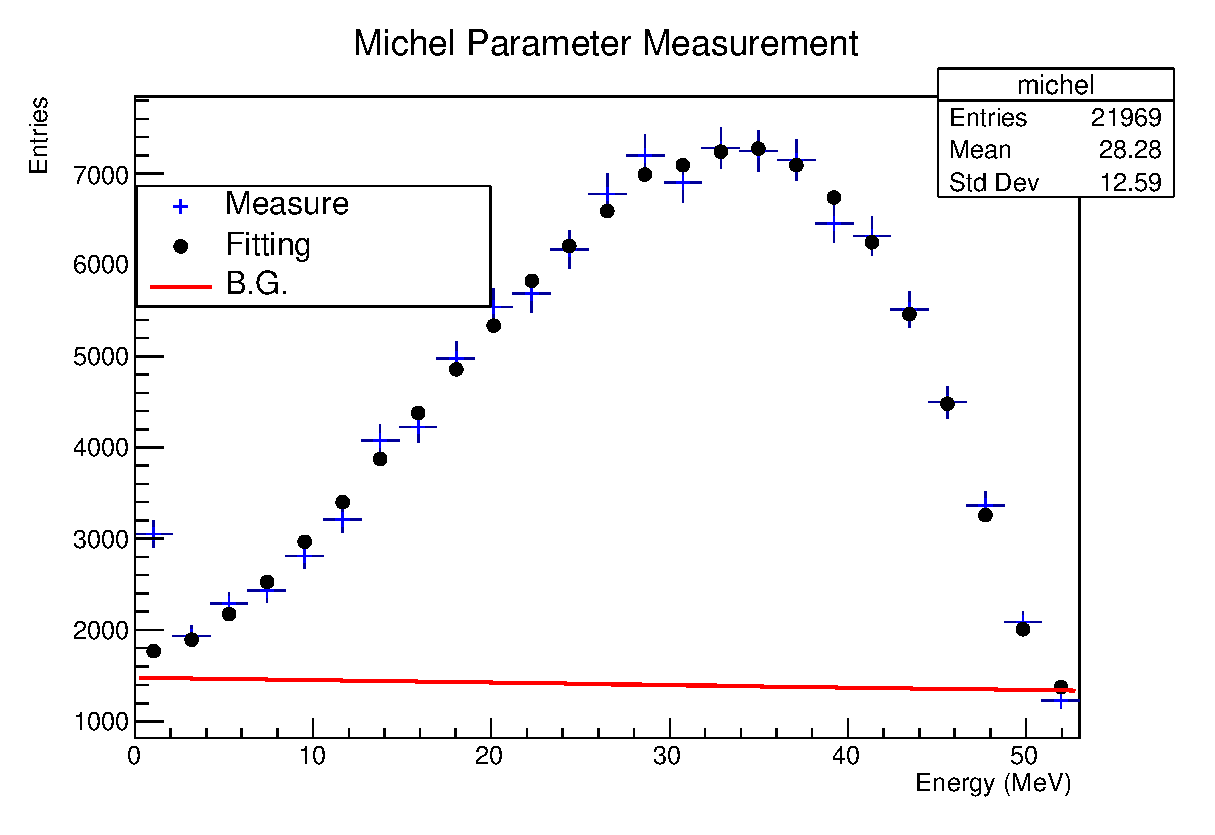
\includegraphics[width=0.8\textwidth]{figure/hatano/rho.eps}
  \caption{$\rho$のFittingの様子}
  \label{hatano_fig:rho}
\end{figure}

\subsubsection{ミッシェルパラメータ$\xi$の導出}
スピンに対する計数の変化を考えると計数はビームが100\%偏極$P_{\mu}=1$なので$\frac{dN}{d\cos\theta}\propto 1+\frac{1}{3}\xi\cos\theta$となり,
スピンが手前を向いている時($0\leq\theta\leq\frac{\pi}{2}$)の計数$N_-$と逆を向いている時($\frac{\pi}{2}\leq\theta\leq\pi$)の計数$N_+$の比を見ると,$\frac{N_+}{N_-}=\frac{1+\frac{1}{6}\xi}{1-\frac{1}{6}\xi}$であるのでこれを求めればよい.これらはスピンの向きに関する部分の測定なので,単純なバックグラウンドだけでなくターゲット内散乱により無偏極となったものによるバックグラウンドも考えなければならない,ただし特に後者の影響を見積もる事は難しいがどちらも$\xi$を小さく見積もる方向に影響を与える.

最初の一周期の該当する範囲で計数を考えると$N_+=73607.5$,$N_-=52878.6$となる.ここでも,指数関数の重みをつけていることを忘れてはいけない.以上より,この比を$R=\frac{N_+}{N_-}$とすると$\xi=6\frac{R-1}{R+1}$より求まり,$\xi=0.983\pm0.017$となる.


\subsubsection{ミッシェルパラメータ$\delta$の導出}
スピンがある方向を向いている時のスペクトラムを見ることにより,残るミッシェルパラメータは$\delta$を含む形で表される.ただし,あるスピンを適当に選び抜き$\delta$を測定するには$\rho$や$\xi$などのパラメータを含む形になりパラメータの数が多くなる.ここで,ちょうどスピンが反対のものを差し引くと$\rho$の関わる部分がキャンセルをし,$\xi$は比例係数の内に含まれるため,$\delta$のみでエネルギースペクトラムは表され,$f(x)\propto(1-\frac{x}{E_{max}})+\frac{2}{3}\delta(4\frac{x}{E_{max}}-3)$と表される.

実際にはスピンが手前を向いている時($0\leq\theta\leq\frac{\pi}{2}$)と逆を向いている時($\frac{\pi}{2}\leq\theta\leq\pi$)を差し引いたスペクトラムに対して
Fittingを行った.$\rho$の導出と同様に較正係数を動かして適切なFittingを決めた.その様子が\figref{hatano_fig:delta}である.またその結果が\tabref{hatano_tab:delta}であり,その結果より$\delta=0.613\pm0.112$である.また系統誤差は最小で0.464,最大で0.794となったので最大幅の0.181とした.すなわち$\delta=0.613\pm0.112\pm0.181$である.
\begin{table}[bht]
  \centering
  \caption{$\delta$のFittingパラメータ}
  \begin{tabular}{cccccccc}
    $p_0$ & $\delta p_0$ & $p_1$ & $\delta p_1$ & $p_2$ & $\delta p_2$ & $p_3$ & $\delta p_3$ \\ \hline
    0.978 & 0.123 & 1.595 & 0.211 & 104.741 & 2.722 & 0.211 & 0.123 \\
  \end{tabular}
  \label{hatano_tab:delta}
\end{table}

\begin{figure}[bht]
  \centering
  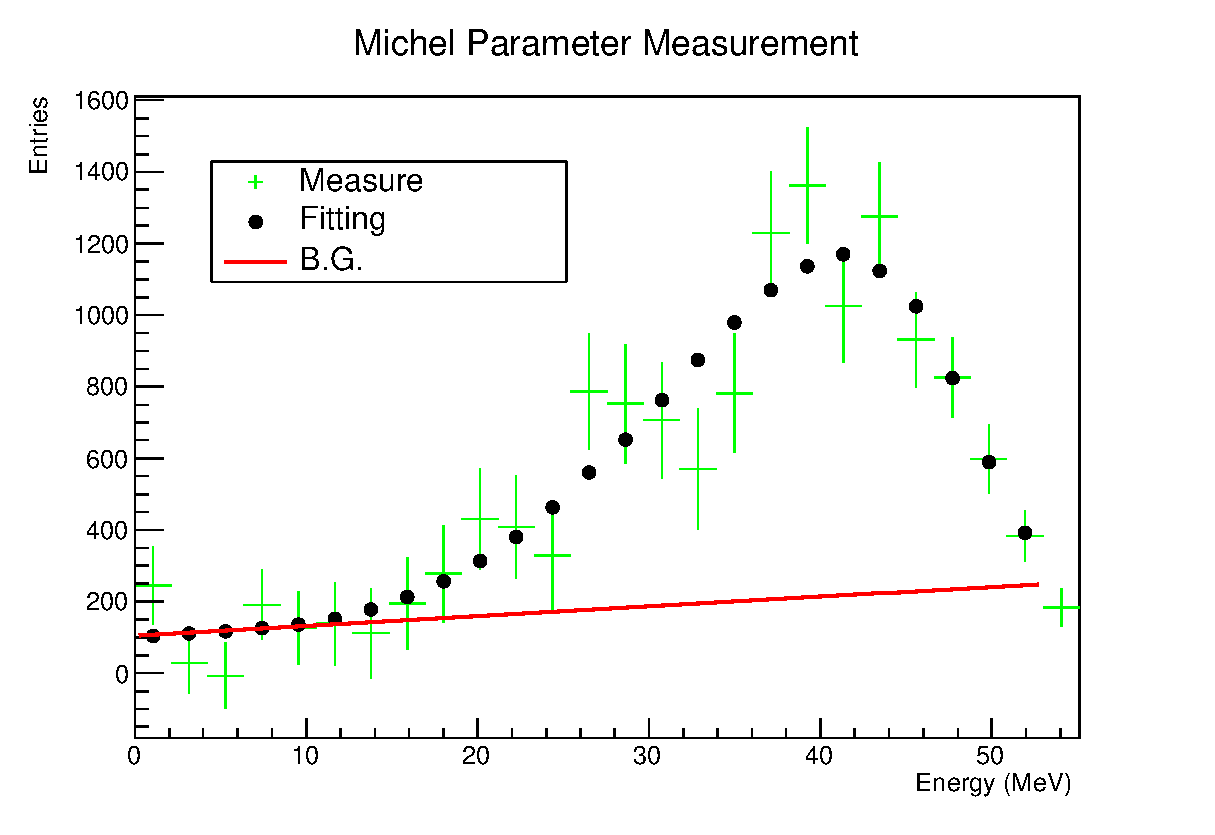
\includegraphics[width=0.8\textwidth]{figure/hatano/delta.eps}
  \caption{$\delta$のFittingの様子}
  \label{hatano_fig:delta}
\end{figure}

\subsection{ミッシェルパラメータのまとめ}
ミッシェルパラメータ$\rho$の値より$\rho=0.75$でベクトル型の相互作用であると考えることが妥当であると分かる.また,$\xi$の測定よりパリティの破れが最大である,V-A理論であるということが分かる.また,$\delta$の測定もベクトル型の相互作用であることを否定しない.以上,測定したミッシェルパラメータをまとめると,\tabref{hatano_tab:michel}となる.

\begin{table}[bht]
  \centering
  \caption{ミッシェルパラメータ結果}
  \begin{tabular}{ccc}
    \hline
    ミッシェルパラメータ & V-A理論 & 測定値 \\ \hline
    $\rho$   & 0.75 & $0.66\pm0.02\pm0.14$ \\
    $\delta$ & 0.75 & $0.61\pm0.11\pm0.18$ \\
    $\xi$    & 1.00 & $0.983\pm0.017$\\
    \hline
  \end{tabular}
  \label{hatano_tab:michel}
\end{table}

%\section{Appendix}
%\subsection{最小二乗法}

%\end{document}
